\documentclass[11pt]{article}
    \title{\textbf{LSDisplacer 0.1.0}}
    \author{Imran Lokhat}
    \date{}
    
    \addtolength{\topmargin}{-3cm}
    \addtolength{\textheight}{3cm}
\usepackage{graphicx}
\usepackage[main=french]{babel}
\usepackage{tikz}
\usepackage{amsmath}
\setcounter{MaxMatrixCols}{15}
\usepackage{minted}
\usepackage{hyperref}

\begin{document}

\maketitle
\thispagestyle{empty}

\section{Introduction}
Le problème considéré est de déplacer/déformer un ensemble de lignes (des talus), par rapport à un réseau d'autres lignes (des routes) pour qu'à une échelle donnée, leurs rendus ne se superposent pas.\\
Un talus est une polyligne, i.e. une suite de points 2D qui forment des segments consécutifs (Figure \ref{points_segments}).\\

\begin{figure}[htp]
	\centering
	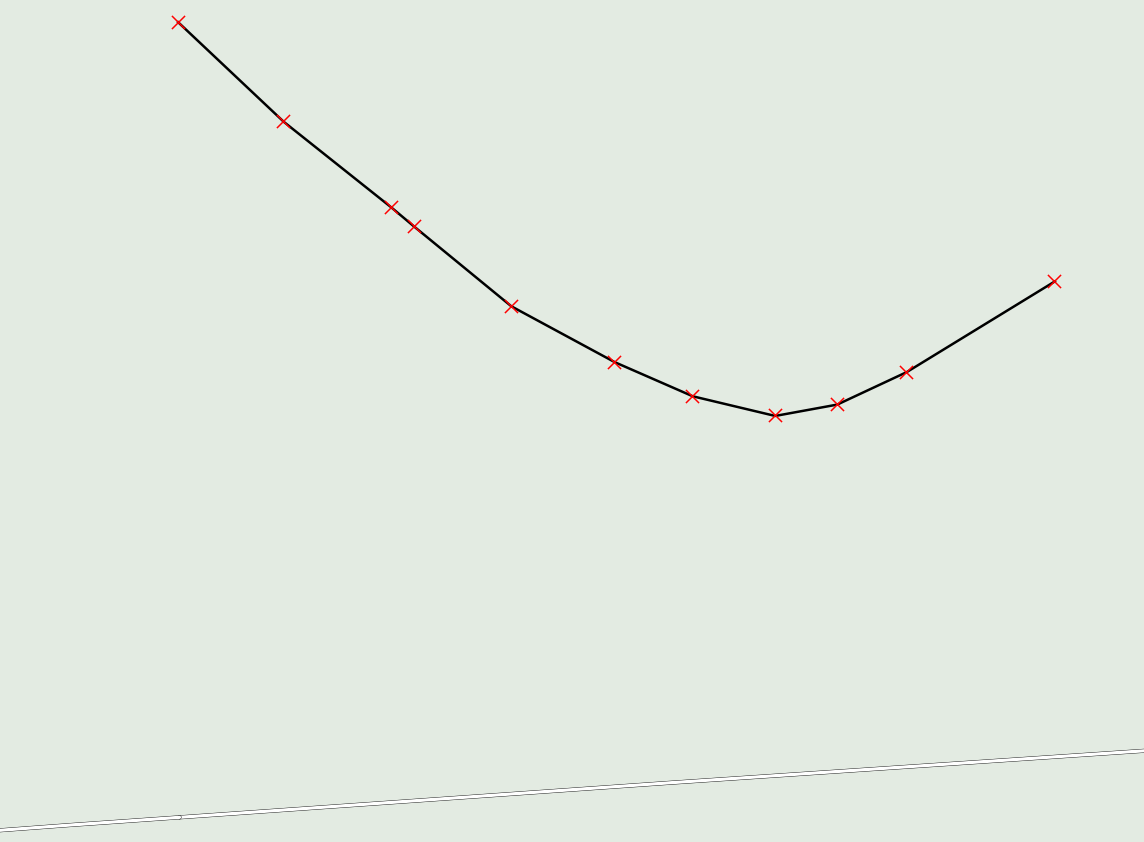
\includegraphics[scale=0.30]{points_segments.png}
	\caption{Points et segments d'un talus}
	\label{points_segments}
\end{figure}

L'échelle est donnée, on sait donc de combien de mètres on cherche à déplacer les talus pour qu'ils soient suffisamment éloignés de l'ensemble des routes en présence.\\
Le processus est local, on est au niveau d'une petite zone correspondant à quelques routes et talus qui forment une unité logique, i.e. un îlot urbain ou un morceau d'îlot (Figure \ref{ilot_talus_routes}).\\
À la fin, on obtient de nouvelles coordonnées pour les points dont sont constitués les talus.\\
\begin{figure}[htp]
	\centering
	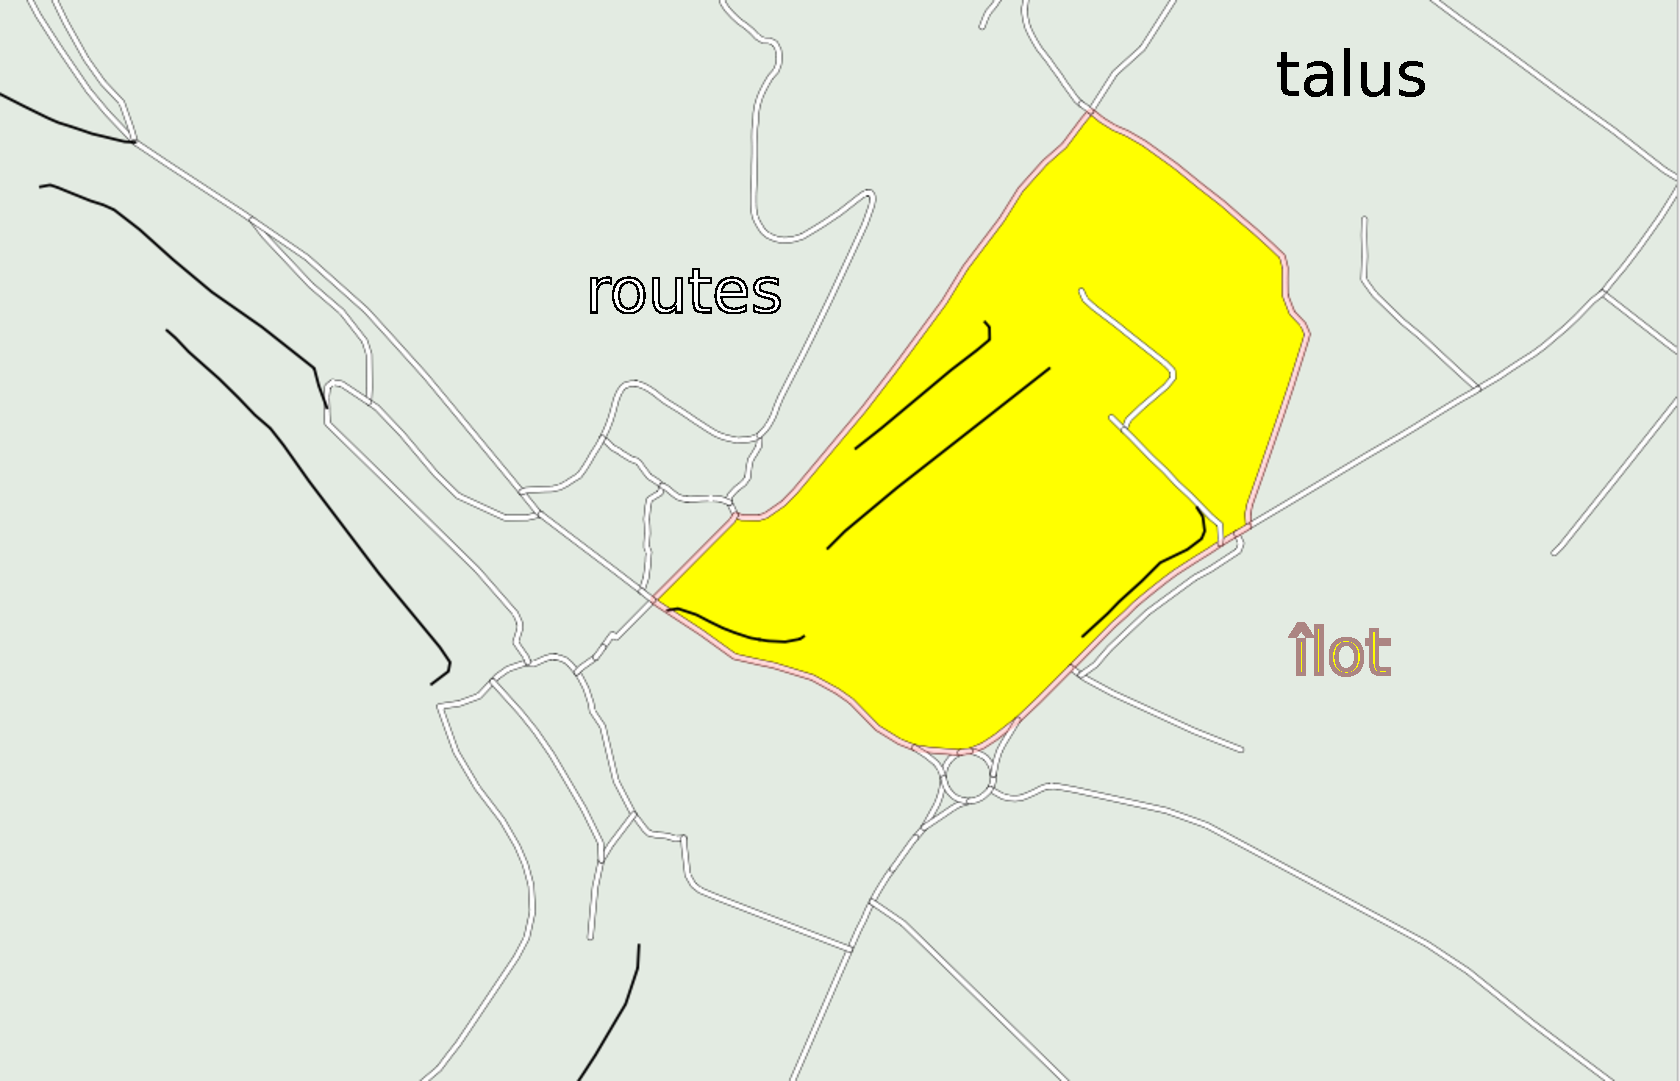
\includegraphics[scale=0.45]{ilot_talus_routes.pdf}
	\caption{Îlot, routes et talus}
	\label{ilot_talus_routes}
\end{figure}


Afin d'essayer de minimiser les déformations spatiales des talus, un certain nombre de contraintes sont exprimées sous forme d'équations portant sur les coordonnées des points, et le système est résolu par moindres carrés.

\section{Moindres carrés non linéaires}
\label{lsq}
Le procédé est itératif, à chaque étape $m$ un vecteur d'incrément $dX^m$ est calculé, qu'on ajoute aux coordonnées courantes $X^{m}$ pour obtenir la nouvelle solution $X^{m+1} = dX^m+X^{m}$.
\
\\
On réitère jusqu'à ce que le critère d'arrêt soit satisfait: 
\begin{itemize}
\item ou bien on a atteint le nombre maximal d'itérations fixé
\item ou alors $\lVert dX^m \rVert_{\infty}$ est inférieure à un seuil donné, i.e. le déplacement est minime suivant toutes les directions
\end{itemize}
\
\\
Le formalisme utilisé est le suivant :
\begin{description}
\addtolength{\itemindent}{0.80cm}
\itemsep0em 
\item[$X^m$] vecteur des coordonnées $(x_0, y_0,\ \dots \ , x_n, y_n)$ des points de l'ensemble des talus à l'itération $m$ (les coordonnées initiales sont donc $X^0$)
\item[$dX^m$] vecteur d'incrément obtenu à la fin de l'itération $m$
\item[$P$] matrice des poids des contraintes
\item[$Y$] vecteur des observations, il contient les valeurs initiales pour les coordonnées des points, les produits vectoriels des angles, les longueurs de segments et autant de 0 que de routes
\item[$S(X^m)$] fonction du modèle, calcule les contraintes pour la solution courante à l'itération m 
\item[$A$] matrice jacobienne du système, i.e. les valeurs des dérivées partielles pour chaque contrainte à l'itération m 
\end{description}
\
Avec $ B = Y - S(X^m)$, les équations normales du système à l'itération $m$  sont :
\begin{displaymath}
(A^TPA) dX^m = A^TPB
\end{displaymath}
 et 
\begin{displaymath}
X^{m+1} = X^m + (A^TPA)^{-1} A^TPB
\end{displaymath}

\section{Contraintes}
Les contraintes, dont la formulation mathématique est $S(X)$, s'appliquent sur les coordonnées des points des talus. Elles cherchent à éloigner les talus des routes de la distance voulue, à minimiser leur déformation (angles et segments internes), et à préserver la figure que forme l'ensemble des talus. 

\subsection{Mouvement}
Les points ne doivent pas trop s'éloigner de leur position d'origine. La contrainte s'exprime trivialement comme :
\begin{equation}
c_i = c_i\  \ \forall c_i \in \lbrace x_0, y_0, \ldots , x_n, y_n \rbrace
\label{movement}
\end{equation}

Il y a autant de contraintes que de coordonnées, soit deux fois le nombre de points.

\subsection{Angles}
Pour un talus donné, on essaie de conserver les angles que forment les segments entre eux.

\begin{center}
\begin{tikzpicture}[scale=0.9]
\coordinate (P0) at (0, 0) ;
\coordinate (P1) at (1.5, 0) ;
\coordinate (P2) at (3, 1) ;
\coordinate (P3) at (4.7, 0.7) ;
\coordinate (P4) at (7.5, 1.2) ;

\draw (P0) -- (P1) node[below] {$P_{i-1}$} -- (P2) node[above] {$P_{i}$} -- (P3) node[below] {$P_{i+1}$} -- (P4) ;
\draw [red, >=latex, ->] (P1) -- (P2) node[midway,above]{$\vec{u}$};
\draw [red, >=latex, ->] (P2) -- (P3) node[midway,above]{$\vec{v}$};
\draw [red] (3.3, 0.94) arc(0:-158:0.3);
\draw [red] (3.1, 0.4) node {$\alpha$};
\draw (P0) node{$\bullet$} ;
\draw (P1) node{$\bullet$} ;
\draw [red] (P2) node{$\bullet$} ;
\draw (P3) node{$\bullet$} ;
\draw (P4) node{$\bullet$} ;
\end{tikzpicture}
\end{center}

En chaque point $P_i$ qui n'est pas une des extrémités du talus, sommet d'un angle $\alpha$, on considère les deux points $P_{i-1}$ et $P_{i+1}$ qui l'entourent, et on calcule le produit vectoriel des deux vecteurs (normés) qui se suivent.
\begin{equation}
C(\alpha) = C(P_{i-1},P_{i}, P_{i+1}) = \frac{\vec{u}}{\lVert \vec{u} \rVert} \times \frac{\vec{v}}{\lVert \vec{v} \rVert} 
\label{crossprod}
\end{equation}

Il y a autant de contraintes qu'il y a d'angles, i.e. le nombre total de points de talus moins deux fois le nombre de talus (on enlève les extrémités de chaque talus).


\subsection{Longueur des segments}
À l'instar des contraintes d'angles, on essaie de conserver les longueurs des segments des talus pour ne pas trop les déformer. On cherche aussi à ne pas trop changer la figure globale formée par l'ensemble des talus.\\
Pour se faire, on va générer une triangulation de Delaunay contrainte (voir figure \ref{triangulation}) entre tous les points de tous les talus, et calculer la longueur de ces segments, i.e. pour deux points de coordonnées $(x_1,y_1)$ et $(x_2, y_2)$ définissant un segment $e$:
\begin{equation}
\text{L(e)} = \sqrt{(x_1 - x_2)^2 + (y_1- y_2)^2}
\label{length_segment}
\end{equation}
\\
\begin{figure}[htp]
\centering
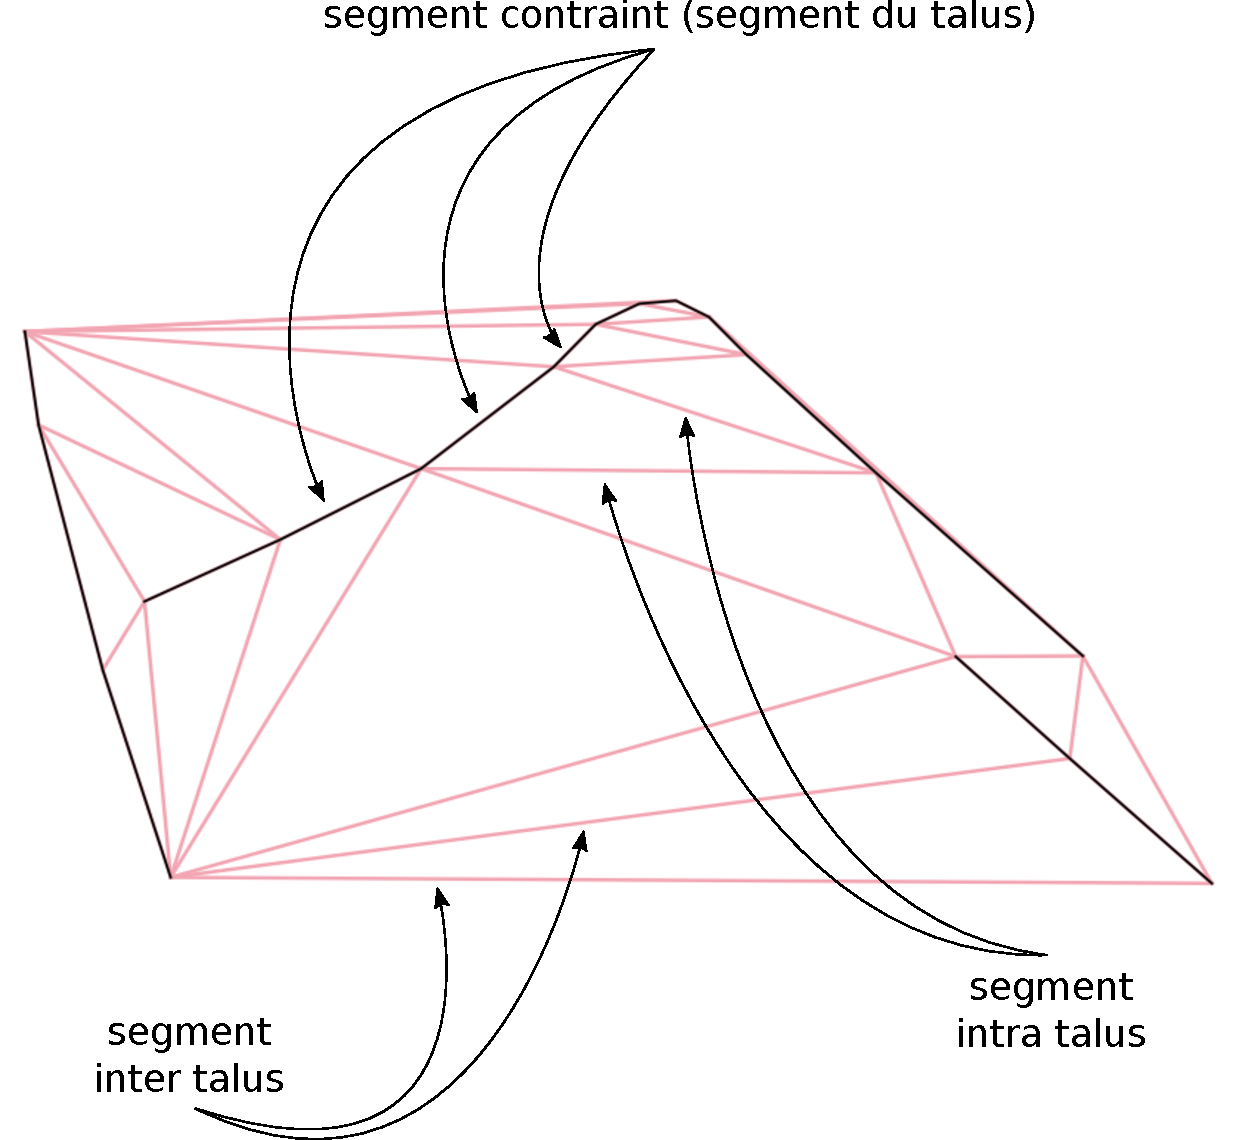
\includegraphics[scale=0.4]{triangulation.pdf}
\caption{Triangulation contrainte entre tous les points de talus}
\label{triangulation}
\end{figure}

Il y a autant de contraintes que de segments issus de la triangulation ($\Theta(\text{nombre de points})$, empiriquement à peu près deux fois le nombre de points).

\subsection{Distance minimale aux routes}

On impose aux points des talus d'être à une distance minimale fixée, disons $\text{\textit{buffer}}_k$,  d'une route $r_k$ donnée.\\
Appelons l'ensembles des talus $\mathbf{T}$, et $dmin_k$ la distance de l'ensemble des polylignes $\mathbf{T}$ à la polyligne $r_k$. \\
On définit alors une fonction $\text{d}_T(r_k)$ :

\begin{equation}
\text{d}_T(r_k) = 
\begin{cases}
\text{buffer}_k - \text{dmin}_k & \text{si dmin}_k < \text{buffer}_k \\
0 &  \text{sinon}
\end{cases} 
\label{dist_route}
\end{equation}


Le nombre de ces contraintes est égal au nombre de routes.

\subsection{Mise en forme matricielle}

\subsubsection{Modèle}
Avec les fonctions qui viennent d'être définies, on note $\_^m$ une donnée à l'itération $m$, et $\_^o$ une donnée initiale.\\
Les $\alpha_i$ sont les sommets de chaque angle d'un talus,  les $e_i$ les segments issus de la triangulation, et les $r_i$ les routes.\\
Nous écrivons alors la matrice $B$ comme :

$$ B = Y - S(X) =
\begin{array}{cc}
	\begin{pmatrix}
	x_0^{o} - x_0^{m}\\y_0^{o} - y_0^{m}\\ \vdots\\ x_n^{o} - x_n^{m}\\ y_n^{o} - y_n^{m}\\
	C(\alpha_0^{o}) - C(\alpha_0^{m})\\ \vdots \\ C(\alpha_j^{o}) - C(\alpha_j^{m})\\
	L(e_0^{o}) - L(e_0^{m})\\ \vdots \\ L(e_k^{o}) - L(e_k^{m})\\
	0 - d_T(r_0)^{m}\\ \vdots \\ 0-d_T(r_l)^{m}\\
	\end{pmatrix}
& 
	\begin{array}{l} 
		  \left. \rule{0pt}{7.5ex} \right\} \text{contrainte de mouvement \eqref{movement}} \\
		  \left. \rule{0pt}{5.5ex} \right\} \text{angles \eqref{crossprod}} \\
		  \left. \rule{0pt}{5.5ex} \right\} \text{longueurs \eqref{length_segment}} \\
		  \left. \rule{0pt}{5.5ex} \right\} \text{distances aux routes \eqref{dist_route}} \\
	\end{array} 
\end{array}
\\
$$

\subsubsection{Matrice jacobienne}
La matrice jacobienne du système est obtenue en calculant les valeurs des dérivées partielles des contraintes, équations \eqref{movement} à \eqref{dist_route}, pour les variables concernées .\\
On notera que comme la fonction de distance à une route (équation \eqref{dist_route}) n'a pas d'expression analytique simple, on a recours à une dérivation numérique, i.e. en chaque coordonnée $c_i$ on calcule :

\begin{equation*}
\frac{\partial dr_k}{\partial c_{i}} = \frac{d_r(X + h_i) - d_r(X - h_i)}{2h_i}
\end{equation*}
\\

La matrice A s'écrit :

$$A=\begin{array}{cc} 
\begin{pmatrix}  
1      & 0      &\ldots &       & & & &          & \ldots & 0 \\
0      & 1      & 0     &\ldots & & & &          &        & \vdots \\
\vdots &        &       &       & & & &          &        & \vdots \\
\vdots &        &       &       & & & &          & 1      & 0 \\
0      & \ldots &       &       & & & & \ldots   & 0      & 1 \\
0      & \ldots & 0 &\frac{\partial C}{\partial x_{i-1}} & \frac{\partial C}{\partial y_{i-1}} & \ldots& \frac{\partial C}{\partial y_{i+1}}& 0 & \ldots & 0 \\
\vdots &        &       &       & & & &          &        & \vdots \\
0      & \ldots & \frac{\partial L}{\partial x_{j-1}} & \frac{\partial L}{\partial y_{j-1}} & \ldots& \frac{\partial L}{\partial y_{j+1}}& 0 & \ldots & & 0 \\
\vdots &        &       &       & & & &          &        & \vdots \\
\frac{\partial dr_0}{\partial x_{0}}  & \ldots & &  & &  & & & \ldots & \frac{\partial dr_0}{\partial y_{n}} \\
\vdots &        &       &       & & & &          &        & \vdots \\       
\frac{\partial dr_l}{\partial x_{0}}  & \ldots & &  & &  & & & \ldots & \frac{\partial dr_l}{\partial y_{n}} \\
\end{pmatrix} 
&  \begin{array}{l} 
\left. \rule{0pt}{8.5ex} \right\} \text{$I_{2(n+1)}$} \\
\left. \rule{0pt}{5ex} \right\} \text{angles}\\
\left. \rule{0pt}{5ex} \right\} \text{longueurs}\\ 
\left. \rule{0pt}{5ex} \right\} \text{distances routes}\\ 
\end{array}\\ 
%\underbrace{\rule{60ex}{0pt}}_{\text{$2n+1$}}
\end{array}$$

\section{Implémentation}

Elle\footnote{\url{https://github.com/ilokhat/embankment_lsq}} est faite en Python, avec les librairies suivantes :
\begin{itemize}
	\item NumPy pour le calcul matriciel et la résolution par moindres carrés
	\item Triangle pour la triangulation de Delaunay contrainte
	\item Shapely et PyGEOS pour les calculs géométriques
	\item Fiona pour l'import des données
\end{itemize}

\subsection{Classe LSDisplacer }
Définie dans le fichier \verb|displacer.py|, c'est le cœur du programme.

La signature de son constructeur est :

\begin{minted}{python}
def __init__(self, points_talus, roads_wkts, talus_lengths, edges, 
             edges_dist_min=10, edges_dist_max=30)
\end{minted}

Paramètres :
\begin{itemize}
	\item \textbf{points\_talus} : tableau numpy de l'ensemble des coordonnées des points de tous les talus en présence $[x_0, y_0, \ldots , x_n, y_n]$
	\item \textbf{roads\_wkts\_and\_buffers} : liste de couples de routes, au format WKT, et de la distance minimale à laquelle un talus doit être de cette route [('LINESTRING..', 15), ('LINESTRING..', 10), ('LINESTRING..', 15)]
	\item \textbf{talus\_lengths} : liste du nombre de points de chaque talus, dans l'ordre des coordonnées passées dans \textit{points\_talus}
	\item \textbf{edges} : liste des segments issus de la triangulation, sous forme de couples (idx($p_1$), idx($p_2$)), avec idx($p_i$) se référant à l'index de l'extrémité $p_i$ du segment parmi les points
	%\item \textbf{buffer} : distance minimale des routes à laquelle un talus doit se situer
	\item \textbf{edges\_dist\_min} : longueur minimale d'un segment liant deux talus
	\item \textbf{edges\_dist\_max} : distance au dessus de laquelle le poids pour la contrainte de conservation de longueur d'un segment liant deux talus devient négligeable
	
\end{itemize}
\

On peut ajuster les paramètres du calcul à l'aide de la méthode de classe :
\begin{minted}{python}
def set_params(MAX_ITER=250, NORM_DX=0.3, H=2.0, DIST='MIN', KKT=False,
       ID_CONST=True, ANGLES_CONST=True, EDGES_CONST=True, DIST_CONST=True,
       PEdges_int=10, PEdges_ext=2, Pedges_ext_far=0, PEdges_int_non_seg=5, 
       PFix=1., PAngles=50, PDistRoads=1000)
\end{minted}

Tous les paramètres ont des valeurs par défaut, il suffit donc de changer seulement ceux que l'on veut :
\begin{itemize}
	\item \textbf{MAX\_ITER} : nombre max d'itérations
	\item \textbf{NORM\_DX} : seuil pour le critère d'arrêt sur la norme de $dX$
	\item \textbf{H} : valeur utilisée pour le calcul de la dérivée numérique de la fonction de distance aux routes (équation \eqref{dist_route})
	\item \textbf{ID\_CONST, ANGLES\_CONST, EDGES\_CONST, DIST\_CONST} : permettent d'activer/désactiver les contraintes de mouvement, angles, longueurs de segments et distances aux routes
	\item \textbf{PFix, PAngles, PDistRoads} : poids sur les contraintes de mouvement, d'angles et de distance aux routes
	\item \textbf{PEdges\_int, PEdges\_int\_non\_seg} : poids sur la contrainte de longueur des segments intra-talus issues de la triangulation (segments liant des points consécutifs et non consécutifs)
	\item \textbf{PEdges\_ext, Pedges\_ext\_far} : poids sur la longueur des arêtes inter-talus (longueur inférieure ou supérieure à \textit{edges\_dist\_max})
	\item DIST : \textbf{obsolète}. Paramètre qui a servi à tester le type de distance calculée pour la contrainte de distance au routes. Si on met autre chose que 'MIN', au lieu de prendre la distance minimale de l'ensemble des talus à une route, on en prend la moyenne. \textbf{Laisser à 'MIN'}
	\item KKT : \textbf{obsolète}. Paramètre qui a servi à tester un moindre carrés contraint\footnote{\label{kkt} Voir par exemple la slide 16 de \    \url{https://stanford.edu/class/engr108/lectures/constrained-least-squares_slides.pdf}} (la contrainte de distance aux routes doit être exactement respectée). N'apporte rien. \textbf{Laisser à False}
\end{itemize}
\

La méthode \textit{square} effectue l'ajustement par moindres carrés.
On peut ensuite récupérer les nouveaux talus en appelant la méthode \textit{get\_linestrings\_wkts}, qui renvoie une liste (un tableau numpy en réalité) des WKT des talus.\\

Ainsi, lancer de manière minimale le programme consiste, une fois les données en entrée récupérées, à changer les paramètres souhaités, instancier \textit{LSDisplacer}, puis faire appel à sa méthode \textit{square} :

\begin{minted}[baselinestretch=1.2, fontsize=\scriptsize,]
{python}
# ...
# on a récupéré les différentes entrées, point_talus, routes, etc..
# ...

LSDisplacer.set_params(MAX_ITER=300, NORM_DX=0.3, 
                       PFix=8.0, PDistRoads=200, PAngles=8, 
                       PEdges_ext=15, Pedges_ext_far=0.5, 
                       PEdges_int=1, PEdges_int_non_seg=1)

displacer = LSDisplacer(points_talus, roads, talus_lengths, edges, buffer=15)
displacer.square()
for talus in displacer.get_linestrings_wkts():
    print(talus)
\end{minted}

\subsection{Détails d'implémentation}
Le code suit assez fidèlement le principe décrit à la section \ref{lsq} page \pageref{lsq} .

\subsubsection{Structures des données}
\label{structures}
La structure la plus importante de ce code est le tableau numpy, i.e. le \textit{ndarray}\footnote{\url{https://numpy.org/doc/stable/reference/arrays.ndarray.html}}, qui est utilisé pour les diverses matrices et vecteurs de la classe.\\

Les coordonnées des, disons, $n+1$ points de l'ensemble des talus sont mis bout à bout et à plat dans un même vecteur \textit{x\_courant} que l'on note ici $X$. Pour pouvoir les différencier on utilise la liste \textit{talus\_lengths} qui contient le nombre de points de chaque talus.\\
Si on appelle $t_0, \ \ldots , \ t_m$ les talus, on a :
$$
X = (x_0, y_0, \ldots, x_n, y_n) =
\begin{bmatrix}
\underbrace{x_0 \ y_0 \ \ldots \ x_k \ y_k }_\textrm{$t_0$} & \ \ldots \ & \underbrace{x_0 \ y_0 \ \ldots \ x_j \ y_j }_\textrm{$t_m$}
\end{bmatrix}
$$

avec  $\text{talus\_lengths} = [\ \text{nombre\_points}(t_0) \ \ldots \   \text{nombre\_points}(t_m)\ ]$\\

et \  $\sum_{i=0}^{m} \ \text{nombre\_points}(t_i) = n+1$ \ . \\

Les segments issus de la triangulation, i.e. l'argument \textit{edges} du constructeur, sont représentés par un tableau numpy de taille $(N, 2)$ où chaque élément est un couple d'index des points définissant ses extrémités.\\
Ainsi, avec le vecteur des points $X$ tel que décrit plus haut, un index $i$ de \textit{edges} se réfère donc aux coordonnées $x_i$ et $y_i$ d'index $2*i$ et $2*i+1$ dans $X$.\\
Par exemple le tableau $[\ [\ 0 \ 2\ ]\ [\ 1 \ 3\ ]\ [\ 4 \ 5\ ]\ ]$ indique qu'il y a 3 segments. \\
Le second, défini par [1 3], lie les points d'index $1$ et $3$ dans la liste de tous les points de talus et c'est donc le segment dont les extrémités ont pour coordonnées $(X[2], X[3])$ et $(X[6], X[7])$ .\\


Le reste de cette partie est consacrée à balayer de manière descendante mais non exhaustive, le code de \textit{LSDisplacer}.

\subsubsection{square}
La méthode \textit{square} consiste essentiellement en une boucle qui calcule $dX$ itérativement et met à jour les coordonnées courantes \textit{x\_courant} : \\
\begin{minted}
[
baselinestretch=1.2,
fontsize=\scriptsize,
]
{python}
def square(self):
	# ...
	alpha = 0.1
	ro = 0.1
	min_dx = np.inf
	norm_float = LSDisplacer.NORM_DX
	for i in range(LSDisplacer.MAX_ITER):
		dx = self.compute_dx()
		self.x_courant += alpha * dx[0]
		normdx = np.linalg.norm(dx[0], ord=np.inf)
		alpha =  (LSDisplacer.H * ro) / (2**0.5 * normdx) if normdx != 0 else 0.1
		min_dx = normdx if normdx < min_dx else min_dx
		if normdx < norm_float : #NORM_DX :
			break
		if LSDisplacer.FLOATING_NORM:
			norm_float = LSDisplacer.NORM_DX if i < 100 else (LSDisplacer.NORM_DX + 2 * min_dx) / 3
	# ...	
	return self.x_courant
\end{minted}

Deux éléments notables :
\begin{itemize}
	\item pour limiter la divergence, on multiplie en réalité $dX$ par un facteur d'amortissement\footnote{\url{https://en.wikipedia.org/wiki/Non-linear_least_squares\#Shift-cutting}} \textit{alpha}
	\item au dessus de 100 itérations, on augmente la valeur du seuil pour le critère d'arrêt sur la norme de $dX$. On fait une moyenne pondérée entre le minimum atteint jusqu'à présent ($\frac{2}{3}$) et la valeur originale de \textit{NORM\_DX} ($\frac{1}{3}$).\\
	Ce comportement est désactivable en passant la valeur de  \textit{LSDisplacer.FLOATING\_NORM} à \textit{False}
\end{itemize}


\subsubsection{compute\_dx}
Rien de particulier, on construit les matrices $A$ et $B$ à chaque itération, et le système est résolu à l'aide de NumPy :
\begin{minted}
[
baselinestretch=1.2,
fontsize=\scriptsize,
]
{python}
import numpy as np
# ...
def compute_dx(self):
	# if LSDisplacer.KKT:
		# obsolète ...
	A = self.get_A()
	B = self.get_B()
	atp = A.T @ self.P 
	atpa = atp @ A
	atpb = atp @ B
	dx = np.linalg.lstsq(atpa, atpb, rcond=None)
	return dx
\end{minted}

\subsubsection{Matrices P, A et B}
Ces matrices sont construites à l'aide des méthodes \textit{get\_X} ($X = A, B\ \text{ou}\ P$) avec la même logique, en empilant les parties liées à chaque type de contrainte.\\
$P$ est créée une fois pour toute lors de l'instanciation alors que les matrices $A$ et $B$ sont elles régénérées à chaque itération, puisqu'elles dépendent de la solution courante.

\begin{minted}
[
baselinestretch=1.2,
fontsize=\scriptsize,
]
{python}
def get_X(self): 
	X = None
	if LSDisplacer.ID_CONST:
		# construire bloc contrainte mouvement
	if LSDisplacer.ANGLES_CONST:
		# construire bloc contrainte angles
		# l'ajouter au bloc précédent
	if LSDisplacer.EDGES_CONST:
		# construire bloc contrainte longueurs segments
		# l'ajouter au bloc précédent
	if LSDisplacer.DIST_CONST:
		# construire bloc contrainte longueurs segments
		# l'ajouter au bloc précédent
	return X # A ou B..
\end{minted}

\subsubsection*{P}

Matrice diagonale, créée par la méthode \textit{get\_P} dont la partie notable est celle où l'on ajoute les poids pour les contraintes sur les segments issus de la triangulation : pour les segments intra-talus on sépare les segments contraints des autres, et pour les segments inter-talus on sépare ceux qui sont proches ou lointains (longueur $>$ \textit{edges\_dist\_max}) :

\begin{minted}
[
baselinestretch=1.2,
fontsize=\scriptsize,
]
{python}
#...
if LSDisplacer.EDGES_CONST:
	wEdges = []
	for i, e in enumerate(self.edges):
		same_talus = num_talus(e[0], self.talus_lengths) == num_talus(e[1], self.talus_lengths)
		non_consecutive_points = abs(e[0] - e[1]) != 1
		if same_talus:
			if non_consecutive_points:
				wEdges.append(LSDisplacer.PEdges_int_non_seg)
			else:
				wEdges.append(LSDisplacer.PEdges_int)
		else:
			if edge_length(e, self.points_talus) >= self.edges_dist_max:
				wEdges.append(LSDisplacer.Pedges_ext_far)
			else:
				wEdges.append(LSDisplacer.PEdges_ext)
	wEdges = np.array(wEdges)
	weights.append(wEdges)
# ...
\end{minted}


\subsubsection*{B}
Matrice colonne, construite par \textit{get\_B} en soustrayant des données originales (coordonnées, produits vectoriels normés des angles, \dots) celles qui sont recalculées pour la solution courante, à l'aide :
\begin{itemize}
	\item de la méthode \textit{angles\_crossprod} pour les produits vectoriels normés
	\item de la fonction \textit{edge\_length}  pour les longueurs de segments
	\item de la méthode \textit{dist\_F\_vectorized} pour les distances aux routes
\end{itemize}


\paragraph{edge\_length}
Calcule la longueur d'un segment défini par le couple de ses extrémités dans \textit{edges} (voir \ref{structures}).

\paragraph{angles\_crossprod}
Rien de particulier, on parcourt la liste des coordonnées en la séparant en talus puis on calcule le produit vectoriel normé des vecteurs entourant chaque point non extrême.

\paragraph{dist\_F\_vectorized}
Une subtilité pour la méthode \textit{dist\_F\_vectorized}, est qu'elle attend en entrée (en sus d'une route) une matrice de points de talus au lieu d'un seule ligne de points. Cela est dû au besoin de performance pour le calcul de la dérivée numérique comme on le verra à la partie suivante (on calcule la distance pour quatre fois le nombre de points, puisqu'on ajoute/retranche un petit $h$ à chaque coordonnée).\\ 
Aussi, on ajoute une dimension au tableau numpy des points de talus avant d'appeler le calcul de distance.\\
L'indice $i$ est l'index de la route dans le tableau de routes/distances passé au constructeur : il permet d'associer la bonne distance à la route traitée :

\begin{minted}
[
baselinestretch=1.2,
fontsize=\scriptsize,
]
{python}
def get_B(self): 
	#...
	# distance from roads
	if LSDisplacer.DIST_CONST:
		r_dists = []
		for i, r in enumerate(self.roads_shapes):
			fk = - self.dist_F_vectorized(r, i, self.x_courant[np.newaxis,:])
			r_dists.append(fk.item())
		# ...
	return b
\end{minted}

La méthode \textit{dist\_F\_vectorized} construit une multiligne par ligne de points de talus et calcule la distance à la route donnée pour chacune de ces multilignes, comme définie en \eqref{dist_route} :

\begin{minted}
[
baselinestretch=1.2,
fontsize=\scriptsize,
]
{python}
def dist_F_vectorized(self, road, i, points_array):
	ml = []
	for c in points_array:
		m = LSDisplacer._multiline_from_points(c, self.talus_lengths)
		ml.append(m)
	ml = np.array(ml)
	dists = pygeos.distance(road, ml)
	dists = np.where(dists > self.buffers[i], 0., self.buffers[i] - dists)
	return dists
\end{minted}

\subsubsection*{A}
Matrice des dérivées partielles, elle est construite par \textit{get\_A}.\\
Le sous-bloc correspondant aux dérivées de la contrainte de mouvement est la matrice identité $I_{2(n+1)}$ pour $(n+1)$ points. Les autres sous-blocs sont générés par :

\begin{itemize}
	\item \textit{cross\_norm\_diff} pour le produit vectoriel normé
	\item  \textit{edge\_length\_diff} pour la longueur des segments
	\item \textit{dist\_F\_diff} pour la dérivée numérique de la distance à une route
\end{itemize}




\paragraph{edge\_length\_diff}
Les dérivées partielles pour la longueur d'un segment (équation \eqref{length_segment}), se calculent par rapport aux coordonnées des sommets du segment, disons $A(x_a, y_a)$ et $B(x_b, y_b)$ et le code de \textit{edge\_length\_diff} n'est qu'une transcription de ces équations :
\begin{align*}
\frac{\partial L}{\partial x_a} &= \frac{x_a - x_b}{ \lvert AB \rvert }\\
\frac{\partial L}{\partial y_a} &= \frac{y_a - y_b}{ \lvert AB \rvert }\\
\frac{\partial L}{\partial x_b} &= \frac{-(x_a - x_b)}{ \lvert AB \rvert }\\
\frac{\partial L}{\partial y_b} &= \frac{-(y_a - y_b)}{ \lvert AB \rvert }
\end{align*}

\
\paragraph{cross\_norm\_diff}
De même, les dérivées partielles pour le produit vectoriel normé (équation \eqref{crossprod}) se calculent par rapport aux coordonnées des 3 points qui définissent l'angle. Le calcul étant plus long et un peu technique, on a fait de la dérivation symbolique avec SymPy pour obtenir les équations implémentées dans \textit{cross\_norm\_diff}.\\
On pourra se référer au fichier \verb|sympy_differentials.py|.

\
\paragraph{dist\_F\_diff}
Pour calculer la dérivée numérique de manière pas trop lente, on va «vectoriser» les calculs de distance : on crée une matrice où chaque ligne $i$ correspond aux coordonnées des points auxquelles on a ajouté (ou retranché) un $h$ à la $i^\text{ème}$ coordonnée.\\
Cela se fait de manière assez élégante en utilisant le \textit{broadcasting} de NumPy. On ajoute (ou retranche) au vecteur de coordonnées courantes une matrice diagonale de $h$ :


$$
\begin{pmatrix}  
x_0  \\  
y_0 \\
\vdots \\
x_n \\
y_n
\end{pmatrix}
\pm
\begin{array}{cc} 
\begin{pmatrix}  
h      & 0      &\ldots &       & & & &          & \ldots & 0 \\
\vdots &        &       &       & & & &          &        & \vdots \\
\vdots &        &       &       & & & &          &       & \vdots \\
0      & \ldots &       &       & & & & \ldots   & 0      & h \\
\end{pmatrix}
=
 \begin{pmatrix}  
 x_0 \pm h & y_0       &\ldots &        & & & &        & \ldots & y_n \\
 x_0       & y_0 \pm h & x_1   & \ldots & & & &        &        & \vdots \\
 \vdots    &           &       &        & & & &        &        & \vdots \\
 x_0       & \ldots    &       &        & & & &        & \ldots & y_n \pm h\\
 \end{pmatrix}
\end{array}$$

Ce qui permet de calculer $ d_r(X \pm h_i) $ en une fois à l'aide de la vectorisation de \textit{pygeos.distance} utilisée dans la méthode \textit{dist\_F\_vectorized} :
\begin{minted}[baselinestretch=1.2, fontsize=\scriptsize,]
{python}
def dist_F_diff(self, road, i):
	# diagonal matrix with H on diagonal
	h = np.eye(self.nb_vars) * self.H
	coords_plus_H = self.x_courant + h
	coords_minus_H = self.x_courant - h
	# seems a bit faster to have 2 np arrays instead of the same one splitted 
	d_plus = self.dist_F_vectorized(road, i, coords_plus_H)
	d_min = self.dist_F_vectorized(road, i, coords_minus_H)
	ds = (d_plus - d_min) / (2 * self.H)
	return ds
\end{minted}

\subsection{Triangulation}

Les fonctions qui gèrent la triangulation et les segments sont regroupées dans le module \verb|triangulation.py|.\\
\textit{LSDisplacer} attend en entrée des segments issus d'une triangulation de Delaunay contrainte effectuée sur l'ensembles des points de tous les talus.\\
Le calcul de cette triangulation est délégué à la librairie \textit{Triangle}, qui n'est qu'un wrapper Python autour de la (rapide) librairie C du même nom de Jonathan Richard Shewchuk.\footnote{\url{http://www.cs.cmu.edu/~quake/triangle.html}}\\

Pour générer les segments, on appelle la fonction :
\begin{minted}[baselinestretch=1.2, fontsize=\scriptsize,]
{python}
def get_edges_from_triangulation(points_talus, talus_lengths, decimate=False)
\end{minted}

Elle attend en entrée un tableau numpy des points de talus, et la liste du nombre de points pour chaque talus, au format présenté dans la section précédente pour \textit{LSDisplacer}.\\
En sortie on obtient une liste de segments, sous la forme décrite précédemment, i.e. une liste de couples d'index des extrémités des points.\\

Le paramètre \textit{decimate} a été utilisé pour tester l'impact de la décimation de certaines arêtes de la triangulation, afin d'en mesurer l'impact sur la vitesse/qualité de l'ajustement.\\
 On a essayé d'éliminer les segments inter-talus ayant pour origine le même point et formant un angle assez petit.
Cependant, aucun effet intéressant n'ayant été observé, ce paramètre est caduc, et laissé à \textit{False}. On garde donc l'ensemble des segments.\\


\subsection{Code utilitaire}
\label{utils}
Les fonctions se trouvant dans \verb|shapes_and_geoms_stuff.py| servent aux divers scénarios d'exemples d'utilisation du code.\\
Elles sont essentiellement utilisées pour lire les données en entrée et les passer à \textit{LSDisplacer} et sont donc fortement liées au format de celles-ci (shapefiles de lignes, etc.).\\
On notera l'utilisation de la bibliothèque Shapely ici, le besoin de vectoriser des calculs n'étant pas présent.

\subsubsection{get\_points\_talus}
\begin{minted}[baselinestretch=1.2, fontsize=\scriptsize,]
{python}
def get_points_talus(shapely_lines)
\end{minted}

Prend en entrée une liste de géométries Shapely de lignes et renvoie un numpy array de l'ensemble des points de ces lignes.

\subsubsection{get\_STRtrees}
\begin{minted}[baselinestretch=1.2, fontsize=\scriptsize,]
{python}
def get_STRtrees(network_file, talus_file)
\end{minted}

Prend en entrée le chemin vers les shapefiles des routes et talus, et construit deux \textit{STRtree}\footnote{\url{https://shapely.readthedocs.io/en/stable/manual.html\#str-packed-r-tree}}, qui vont permettre d'avoir un index spatial rapide sur les deux collections de lignes.\\

Ce qui va permettre d'accélérer la sélection de routes ou de talus, pour un îlot donné.

\subsubsection{get\_talus\_inside\_face}
\begin{minted}[baselinestretch=1.2, fontsize=\scriptsize,]
{python}
def get_talus_inside_face(f, ttree, merge=True, displace=True)
\end{minted}

Prend en entrée un polygone $f$ représentant un îlot urbain, le \textit{STRtree} des talus, et renvoie les intersections de tous les talus et de cet îlot.\\
Si \textit{merge} est à \textit{True}, on essaie de fusionner les talus consécutifs en un seul talus. \\
Si \textit{displace} est à \textit{True}, on essaie de déplacer les talus qui sont sur la frontière de l'îlot à l'intérieur, soit en les bougeant vers le centroïde de la face si c'est possible, ou alors de manière aléatoire.
\subsubsection{get\_roads\_for\_face}
\begin{minted}[baselinestretch=1.2, fontsize=\scriptsize,]
{python}
def get_roads_for_face(f, ntree, merge=True)
\end{minted}

Fonction symétrique à la précédente, mais pour les routes. On récupère toutes les routes composant l'îlot urbain formé par le polygone $f$, en essayant d'en fusionner le maximum si \textit{merge} est à \textit{True}. En particulier, la frontière extérieure de $f$ mais aussi les frontières des éventuels trous à l'intérieur de $f$ forment chacune une seule route.

\subsection{Exemples d'utilisation}

Le dépôt comporte quelques exemples d'utilisation de la classe \textit{LSDisplacer}.

\subsubsection{main\_simple\_example.py}

Exemple basique d'utilisation : les routes et talus sont des listes de Linestrings au format WKT qu'on charge avec \textit{Shapely}. \\
Le programme est explicite, et suffisamment court pour être reproduit ici :
\begin{minted}[baselinestretch=1.2, fontsize=\scriptsize,]
{python}
from shapely.wkt import loads
from shapes_and_geoms_stuff import get_points_talus
from triangulation import get_edges_from_triangulation
from displacer import LSDisplacer

roads = [('LineString(...)', 10), ('LineString(...)', 20)]
talus = ['LineString(...)', 'LineString(...)', 'LineString(...)']

talus_shapes = [loads(t) for t in talus]
talus_lengths = [len(t.coords) for t in talus_shapes]

points_talus = get_points_talus(talus_shapes)
edges = get_edges_from_triangulation(points_talus, talus_lengths)

LSDisplacer.set_params(MAX_ITER=500, NORM_DX=0.3,
                       PFix=8.0, PDistRoads=200, PAngles=8,
                       PEdges_ext=15, Pedges_ext_far=0.5, 
                       PEdges_int=1, PEdges_int_non_seg=1)

displacer = LSDisplacer(points_talus, roads, talus_lengths, edges)
print("P matrix size", displacer.P.shape)
displacer.square()
displacer.print_linestrings_wkts()
\end{minted}


\subsubsection{main\_by\_faces\_example.py}
Ici, on a un ensemble d'îlots sous forme d'un shapefile de polygones, et on utilise les fonctions utilitaires présentées en \ref{utils} pour récupérer routes et talus pour chaque îlot.\\
Le programme illustre aussi l'utilisation du \textit{logger} de la classe basé sur le module \textit{logging} de la librairie standard : les niveaux utilisés ici, par ordre croissant de sévérité, \textit{DEBUG}, \textit{INFO} et \textit{WARNING}, sont par verbosité décroissante (\textit{DEBUG} est le niveau le plus verbeux). Par défaut on est au niveau \textit{INFO}.


\subsubsection{multiproc\_expe.py}
Variation du programme précédent en version multi-cœurs. Chaque îlot est traité par une unité de calcul disponible.\\
De plus, on partitionne les îlots en groupes de talus proches (leurs distances sont inférieures ou égales à \textit{edges\_dist\_max}) et on ne récupère que les routes concernées afin de réduire la taille des matrices et le nombre de routes impliquées dans les calculs de distances.

\end{document}
